\section{Ontwerp en realisatie IIR filter}

\subsection{Requirements IIR filter}
Het IIR filter moet een Band-Stop filter worden. De minimale orde die verwacht wordt is er een van 20. Het filter moet alle frequenties tussen 800 en 1000 hertz dempen. Het type Chebyshev I zal worden toegepast.
\subsection{Coefficienten bepalen}

\begin{enumerate}[label=\emph{\alph*)}]
    \litem{Orde} teruggeschroeft naar 4 om het filter met een elkele sectie stabiel te krijgen.
    \litem{Fsample} teruggeschroeft om het filter stabiel te krijgen.
    \litem{Fixed-point} getallen gebruikt omdat deze geschikt zijn voor de EzDSP. Deze bevat voor Floating-point getallen namelijk geen hardware ondersteuning.
\end{enumerate}

Er drijgde een gebrek aan tijd tijdens het uitvoeren van de laatste opdracht, hierdoor was het niet meer mogelijk om ondersteuning te maken voor een filter dat bestaat uit meerdere secties. 
Daarop is in oveleg met Dhr. Broeders besloten om een filter te maken dat uit een enkele sectie bestaat. Hiervoor hebben we de orde echter moeten terugschroeven, maar dit was dit geval geen probleem mits dit in het verslag werd beschreven. 

\subsection{Matlab}

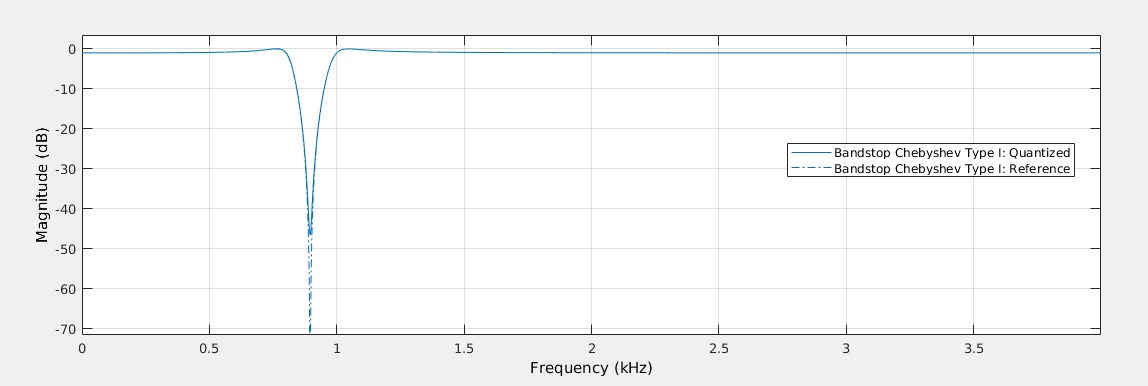
\includegraphics[width=0.80\textwidth]{iirMatlab}\par\vspace{1cm}		
\clearpage
\subsection{Code}

\subsubsection{de main code.}
\begin{lstlisting}[language=c]
#include <stdio.h>
#include <usbstk5505.h>
#include <usbstk5505_led.h>
#include <csl_intc.h>
#include <iir_buffer.h>
#include "aic3204.h"
#include "iir_fdacoefs3.h"

#define SAMPLES_PER_SECOND 8000 // possible values: 48000, 24000, 16000, 12000, 9600, and 8000
#define ADC_GAIN  0// range: 0dB to 48 dB
#define DAC_GAIN 0// range: -6dB to 29dB


extern void VECSTART(void);

 
IIRBuffer *buffer;
interrupt void I2S0receive() {
iir_buffer_store_sample(buffer, AIC3204_readLeft());
AIC3204_writeLeft(iir_buffer_output_sample(buffer, DEN, NUM));

}

int main(void) {
buffer = iir_buffer_new(COEFFICIENTS_LENGTH, 1);

USBSTK5505_init();
AIC3204_init(SAMPLES_PER_SECOND, ADC_GAIN, DAC_GAIN);
IRQ_setVecs((Uint32)(&VECSTART));
IRQ_plug(PROG1_EVENT,&I2S0receive);
IRQ_enable(PROG1_EVENT);
IRQ_globalEnable();

while(1);
}
\end{lstlisting}
\clearpage

\subsubsection{IIR buffer header}
\begin{lstlisting}[language=c]
#ifndef __IIR_BUFFER__
#define __IIR_BUFFER__

#include <csl_intc.h>

typedef struct {
int size;
int sections;
Int16 *buffer;
Int32 *outputBuffer;
int currentBufferIndex;
} IIRBuffer;

IIRBuffer * iir_buffer_new(int size, int sections);
void iir_buffer_store_sample(IIRBuffer *buffer, Int16 sample);
Int16 iir_buffer_output_sample(IIRBuffer *buffer, const Int16 *denominator, const Int16 *numerator);

#endif//__IIR_BUFFER__
    
\end{lstlisting}
\clearpage

\subsubsection{IIR buffer source}
\begin{lstlisting}[language=c]
#include <iir_buffer.h>
#include <stdlib.h>

Int32 direct_form_1(IIRBuffer *buffer, Int32 input, const Int16 *denominator, const Int16 *numerator) {
Int32 output = input;
int k;
for(k = 0; k < buffer->size; k++){
    int bufferIndex = buffer->currentBufferIndex - k;
    if(bufferIndex < 0){
        bufferIndex += buffer->size;
    }

    output += (Int32)numerator[k] * (Int32)buffer->buffer[bufferIndex];
}

int i;
for(i = 1; i < buffer->size; i++) {
    int bufferIndex = buffer->currentBufferIndex - i;
    if(bufferIndex < 0){
        bufferIndex += buffer->size;
    }

    output -= (Int32)denominator[i] * (Int32)buffer->outputBuffer[bufferIndex];
}
return output;
}

IIRBuffer * iir_buffer_new(int size, int sections) {
IIRBuffer *iirBuffer = (IIRBuffer *)malloc(sizeof(IIRBuffer));
//TODO: Still have to solve potential nullpointer issues.

iirBuffer->size = size;
iirBuffer->sections = sections;
iirBuffer->buffer = malloc(sizeof(Int16) * size);
iirBuffer->outputBuffer = malloc(sizeof(Int32) * size);

int i;
for(i = 0; i < size; i++) {
    iirBuffer->buffer[i] = 0;
    iirBuffer->outputBuffer[i] = 0;
}

iirBuffer->currentBufferIndex = 0;

return iirBuffer;
}

void iir_buffer_store_sample(IIRBuffer *buffer, Int16 sample) {
buffer->currentBufferIndex += 1;

if(buffer->currentBufferIndex == buffer->size) {
        buffer->currentBufferIndex = 0;
}

buffer->buffer[buffer->currentBufferIndex] = sample;
}

Int16 iir_buffer_output_sample(IIRBuffer *buffer, const Int16 *denominator, const Int16 *numerator) {
Int32 output = 0;

output += direct_form_1(buffer, output, denominator, numerator);

buffer->outputBuffer[buffer->currentBufferIndex] = output >> 13;
return((Int16)(output>>13));
}
\end{lstlisting}
\clearpage

\subsubsection{IIR coefficients}
\begin{lstlisting}[language=c]
/*
* Filter Coefficients (C Source) generated by the Filter Design and Analysis Tool
* Generated by MATLAB(R) 9.2 and the DSP System Toolbox 9.4.
* Generated on: 23-Oct-2017 14:07:54
*/

/*
* Discrete-Time IIR Filter (real)
* -------------------------------
* Filter Structure    : Direct-Form I
* Numerator Length    : 5
* Denominator Length  : 5
* Stable              : Yes
* Linear Phase        : No
* Arithmetic          : fixed
* Numerator           : s16,13 -> [-4 4)
* Denominator         : s16,13 -> [-4 4)
* Input               : s16,15 -> [-1 1)
* Output              : s16,15 -> [-1 1)
* Numerator Prod      : s32,28 -> [-8 8)
* Denominator Prod    : s32,28 -> [-8 8)
* Numerator Accum     : s40,28 -> [-2048 2048)
* Denominator Accum   : s40,28 -> [-2048 2048)
* Round Mode          : convergent
* Overflow Mode       : wrap
* Cast Before Sum     : true
*/

/* General type conversion for MATLAB generated C-code  */
/* 
* Expected path to tmwtypes.h 
* /usr/local/MATLAB/R2017a/extern/include/tmwtypes.h 
*/
#define COEFFICIENTS_LENGTH 5
const Int16 NUM[5] = {
6735, -20550,  29146, -20550,   6735
};

const Int16 DEN[5] = {
8192, -23961,  32617, -22154,   7008
};	   
\end{lstlisting}
\clearpage

\subsection{Het resultaat}	
    Om het fir-filter dat is gerealiseerd te testen is een functiegenerator gebruikt om een bepaald frequentieberijk te sweepen. Dit bereik was van 100 tot 4000 hertz. De tijd dat deze sweep daarover deed varieerde iets omdat anders gaten vielen in de peak-hold methode van de scope. De uitgang van de EzDSP wedr aangesloten op de microfoonaansluiting van een pc. Op deze pc werd het Soundcard Oscilloscope programma uitgevoerd om de uitvoer te bekijken. Op deze manier kon een hogere Signal to Noise ratio worden gemeten dan met de echte oscilloscopen die aanwezig waren. 
    \\\\Hieronder ziet u een screenshot van dit programma met daarop een frequentie analyze.
    \\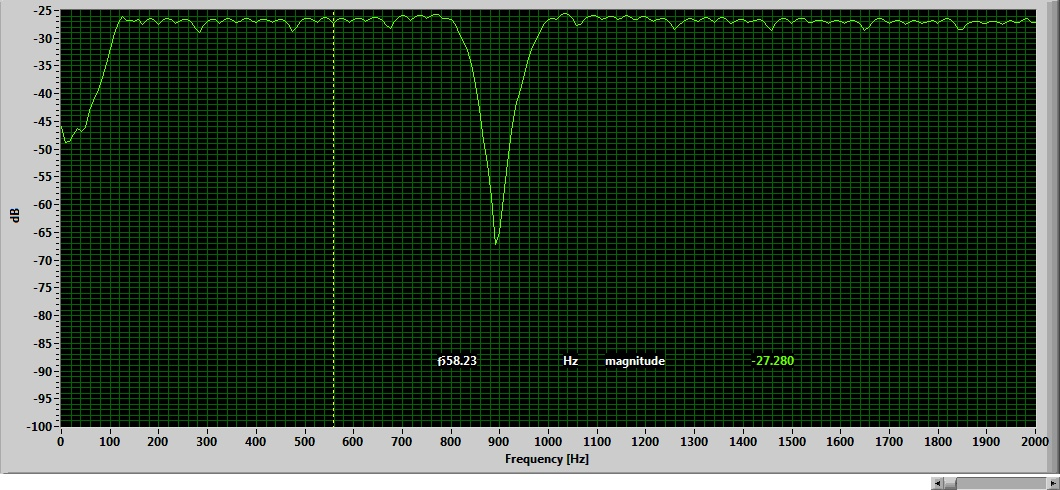
\includegraphics[width=0.80\textwidth]{IIRrealisatie}\par\vspace{1cm}
    Wanneer er een probleem zou zijn met een IIR filter is dat meteen zichtbaar omdat het filter zich dan totaal niet gedraagd zoals gewenst is, maar in dit geval ziet u duidelijk dat hij overheen komt met de voorspelling van Matlab.
    
\clearpage